\documentclass[8pt]{article} % use larger type; default would be 10pt

%\usepackage[utf8]{inputenc} % set input encoding (not needed with XeLaTeX)
\usepackage{graphicx}
\usepackage{float}
\usepackage{subfig}
\usepackage{amsmath}
\usepackage{amsfonts}
\usepackage{graphicx}
\usepackage{mathtools}
\usepackage{hyperref}
\usepackage{harpoon}
\usepackage{enumitem}
\usepackage{multicol}
\usepackage[neverdecrease]{paralist}
\usepackage{enumerate}
\usepackage{cancel}
\usepackage{ulem}

\usepackage{mystyle}

\title{Math 1540\\University Mathematics for Financial Studies\\2013-14 Term 1\\Suggested solutions for\\
HW problems Sec. 2.3-2.4 (Linear Algebra) and Sec. 14.1 (Calculus)}
\begin{document}
\maketitle
\section{Section 2.3 (Linear Algebra)}
\begin{description}
	\item[\# 5.]{{\it Let} \[A=\begin{bmatrix}a&b&c\\d&e&f\\g&h&i\end{bmatrix}\]
	\textit{Assuming that $\det(A)=-7$, find}\\\\
	\begin{inparaenum}[(a)]
		\item $\det(3A)$\qquad
		\item $\det(A^{-1})$\qquad
		\item $\det(2A^{-1})$\qquad
		\item $\det((2A)^{-1})$\qquad
		\item $\det\begin{bmatrix}a&g&d\\b&h&e\\c&i&f\end{bmatrix}$
	  \end{inparaenum}\\\\
	\begin{enumerate}[(a)]
	\item \[\det(3A)=\begin{vmatrix}3a&3b&3c\\3d&3e&3f\\3g&3h&3i\end{vmatrix}=
	3\cdot\begin{vmatrix}a&b&c\\3d&3e&3f\\3g&3h&3i\end{vmatrix}=
	3\cdot3\cdot\begin{vmatrix}a&b&c\\d&e&f\\3g&3h&3i\end{vmatrix}=\]\[=
	3\cdot3\cdot3\cdot\begin{vmatrix}a&b&c\\d&e&f\\g&h&i\end{vmatrix}=3\cdot3\cdot3\cdot(-7)=-189\]
	\item As we have \[\det(A)\det(A^{-1})=\det(AA^{-1})=\det(I)=1\] we conclude \[\det(A^{-1})=\frac{1}{\det(A)}=-\frac{1}{7}\]
	\item Similarly to the first subproblem \[\det(2A^{-1})=2\cdot2\cdot2\det(A^{-1})=-\frac{8}{7}\]
	\item As \[(2A)\cdot(\frac{1}{2}A)=2\cdot\frac{1}{2}AA^{-1}=I\] we conclude that $(2A)^{-1}=\frac{1}{2}A^{-1}$ and hence
	\[\det((2A)^{-1})=\det(\frac{1}{2}A^{-1})=\frac{1}{2}\cdot\frac{1}{2}\cdot\frac{1}{2}\cdot\det(A^{-1})=-\frac{1}{56}\]
	\item 
		\[\begin{array}{rr}
		\begin{vmatrix}a&g&d\\b&h&e\\c&i&f\end{vmatrix}= &\mbox{ (\textit{transposing does not change determinant}) }\\\\
		=\begin{vmatrix}a&b&c\\g&h&i\\d&e&i\end{vmatrix}= &\mbox{ (\textit{interchanging rows changes sign}) }\\\\
			=-\begin{vmatrix}a&b&c\\d&e&i\\g&h&i\end{vmatrix}=&-\det(A)=7
		\end{array}\]
	\end{enumerate}
	}
	\item[\# 7.]{{\it Without directly evaluating, show that}
		\[\det\begin{bmatrix}b+c&c+a&b+a\\a&b&c\\1&1&1\end{bmatrix}=0\]
		This is not difficult
		\[\begin{array}{rr}
		\begin{vmatrix}b+c&c+a&b+a\\a&b&c\\1&1&1
		\end{vmatrix}= &\mbox{ (\textit{adding row to row does not alter determinant})}\\\\
		=\begin{vmatrix}b+c+a&c+a+b&b+a+c\\a&b&c\\1&1&1
		\end{vmatrix}= &\mbox{ (\textit{scaling one row scales the determinant})}\\\\
		=(a+b+c)\cdot\begin{vmatrix}1&1&1\\a&b&c\\1&1&1
		\end{vmatrix}= &\mbox{ (\textit{matrix with identical rows has zero determinant})}\\\\
		=(a+b+c)\cdot0=0&\end{array}\]
		}
	\item[\# 17.]{{\it \begin{enumerate}[(a)]
			\item Express\[\begin{vmatrix}a_1+b_1&c_1+d_1\\a_2+b_2&c_2+d_2\end{vmatrix}\] as a sum of four determinants
					whose entries contain no sums
		\end{enumerate}
		}
		\begin{enumerate}[(a)]
			\item 
		\[\begin{array}{rr}
		\begin{vmatrix}a_1+b_1&c_1+d_1\\a_2+b_2&c_2+d_2\end{vmatrix}= &\mbox{ (\textit{determinant is linear in first row})}\\\\
		=\begin{vmatrix}a_1&c_1\\a_2+b_2&c_2+d_2\end{vmatrix}+
		\begin{vmatrix}b_1&d_1\\a_2+b_2&c_2+d_2\end{vmatrix}
			= &\mbox{ (\textit{determinant is linear in second row})}\\\\
		=\begin{vmatrix}a_1&c_1\\a_2&c_2\end{vmatrix}+
		\begin{vmatrix}a_1&c_1\\b_2&d_2\end{vmatrix}+
		\begin{vmatrix}b_1&d_1\\a_2&c_2\end{vmatrix}+
			\begin{vmatrix}b_1&d_1\\b_2&d_2\end{vmatrix}\end{array}
		\]
		\end{enumerate}
		}
	\item[\# 18.]{{\it Prove that a square matrix is invertible if and only if $A^TA$ is invertible.
				}
			Assume that $A$ is invertible. Then, $A^T(A^{-1})^T=(A^{-1}A)^T=I^T=I$, so $A^T$ is also invertible and hence
			$A^TA$ is invertible as a product of invertible matrices.

			Conversely, suppose $A^TA$ is invertible. Then $0\neq \det(A^TA)=\det(A^T)\det(A)=\det(A)\cdot\det(A)\implies
			\det(A)\neq 0$ and hence $A$ is invertible.
				}
\section{Section 2.4 (Linear Algebra)}
\newcommand{\mymat}[2]{\mysbra{\begin{array}{#1}#2\end{array}}}
\newcommand{\adj}{\mbox{adj}}
	\item[\# 4.]{{\it For the matrix \[A=\mymat{rrr}{1&-2&3\\6&7&-1\\-3&1&4}\]
		find\\\\
		\begin{inparaenum}[(a)]
		\item $\adj(A)$\qquad
		\item $A^{-1}$ using Theorem 2.4.2
		\end{inparaenum}\\\\
		}
		This problem is straightforward
		\begin{enumerate}[(a)]
			\item \[\adj(A)=\left[\begin{array}{rrr}
					+\det(M_{1,1}) & -\det(M_{2,1})&+\det(M_{3,1})\\
					-\det(M_{1,2}) & +\det(M_{2,2})&-\det(M_{3,2})\\
					+\det(M_{1,3}) & -\det(M_{2,3})&+\det(M_{3,3})\\
				\end{array}\right]=\]
				\[=\left[\begin{array}{rrr}
					29&11&-19\\
					-21&13&19\\
					27&5&19
				\end{array}\right]\]
				Here by $M_{i,j}$ we denote matrix $A$ with row $i$ and column $j$ cut out, as usual. 
				Just as a recap, let us write down the computation of $\det(M_{3,2})$
				\[\det(M_{3,2})=\left|\begin{array}{rrr}1& \cancel{-2}& 3\\
					6& \cancel{7}& -1\\
					\cancel{-3}& \cancel{1}& \cancel{4}\\
				\end{array}\right|=\left|\begin{array}{rr}1& 3\\
					6& -1\\
				\end{array}\right|=1\cdot(-1)-6\cdot3=-19\]
			\item Knowing the adjoint matrix, it easy to explicitly write down the inverse
				\[A^{-1}=\frac{1}{\det(A)}\adj(A)=\frac{1}{152}
				\left[\begin{array}{rrr}
					29&11&-19\\
					-21&13&19\\
					27&5&19
				\end{array}\right]\]
				as
				\[
				\det(A)=\left|\begin{array}{rrr}
					1&-2&3\\6&7&-1\\-3&1&4
				\end{array}\right|=
				\left|\begin{array}{rrr}
					1&-2&3\\0&19&-19\\0&-5&13
				\end{array}\right|=
				19\left|\begin{array}{rrr}
					1&-2&3\\0&1&-1\\0&0&8
				\end{array}\right|=19\cdot1\cdot1\cdot8=152
				\]
		\end{enumerate}
		}
	\item[\# 17.]{{\it Solve by Cramer's Rule, if it applies\\\\
			$\begin{array}[t]{rrrrrrr}
				4x & + {} & 5y & & & = & 2\\
				11x & + {} & y & + {} & 2z& = & 3\\
				x & + {} & 5y & + {} & 2z& = & 1
			\end{array}$\\\\
			}Rewriting the equation in matrix form we have
			\[A\mathbf{x}=
			\begin{bmatrix}4&5&0\\11&1&2\\1&5&2\end{bmatrix}\begin{bmatrix}x\\y\\z\end{bmatrix}=\begin{bmatrix}2\\3\\1\end{bmatrix}=
				\mathbf{b}\]
			Hence
			\[A=\begin{bmatrix}4&5&0\\11&1&2\\1&5&2\end{bmatrix},\quad \mathbf{b}=\begin{bmatrix}2\\3\\1\end{bmatrix}\]
			To begin with,
			\[\begin{array}{rr}
			\det(A)=\begin{vmatrix*}[r]4&5&0\\11&1&2\\1&5&2\end{vmatrix*}
			= &\mbox{ (\textit{interchanging 1st and 3rd row changes sign})}\\\\
			=-\begin{vmatrix*}[r]1&5&2\\11&1&2\\4&5&0\end{vmatrix*}=
			&\mbox{ (\textit{subtracting first row from another does not change determinant})}\\\\
			=-\begin{vmatrix*}[r]1&5&2\\0&-54&-20\\0&-15&-8\end{vmatrix*}=
			&\mbox{ (\textit{expand along the first column})}\\\\
			=-\begin{vmatrix*}[r]-54&-20\\-15&-8\end{vmatrix*}=&-((-54)\cdot(-8)-(-15)\cdot(-20))=15\cdot20-54\cdot8=-132
			\end{array}\]
			Hence $\det(A)\neq 0$, thus Cramer's Rule applies. Proceeding, we have
			\[\begin{array}{rr}
			\det(A_1)=\begin{vmatrix*}[r]\mathbf{2}&5&0\\\mathbf{3}&1&2\\\mathbf{1}&5&2\end{vmatrix*}
			= &\mbox{ (\textit{subtracting third row from others does not change determinant})}\\\\
			=\begin{vmatrix*}[r]0&-5&-4\\0&-14&-4\\{1}&5&2\end{vmatrix*}
			= &\mbox{ (\textit{expand along the first column})}\\\\
			=1\cdot
			\begin{vmatrix*}[r]-5&-4\\-14&-4\end{vmatrix*}=&(-5)\cdot(-4)-(-14)\cdot(-4)=-36\implies x=\frac{\det(A_1)}{\det(A)}=
				\frac{-36}{-132}=\frac{3}{11}
			\end{array}\]

			\[\begin{array}{rr}
			\det(A_2)=\begin{vmatrix*}[r]4&\mathbf{2}&0\\11&\mathbf{3}&2\\1&\mathbf{1}&2\end{vmatrix*}
			= &\mbox{ (\textit{subtracting third row from others does not change determinant})}\\\\
			=\begin{vmatrix*}[r]0&-2&-8\\0&-8&-20\\1&{1}&2\end{vmatrix*}
			= &\mbox{ (\textit{expand along the first column})}\\\\
			=1\cdot
			\begin{vmatrix*}[r]-2&-8\\-8&-20\end{vmatrix*}=&(-2)\cdot(-20)-(-8)\cdot(-8)=-24\implies y=\frac{\det(A_2)}{\det(A)}=
				\frac{-24}{-132}=\frac{2}{11}
			\end{array}\]

			\[\begin{array}{rr}
			\det(A_3)=\begin{vmatrix*}[r]4&5&\mathbf{2}\\11&1&\mathbf{3}\\1&5&\mathbf{1}\end{vmatrix*}
			= &\mbox{ (\textit{subtracting third row from others does not change determinant})}\\\\
			=\begin{vmatrix*}[r]0&-15&{-2}\\0&-54&{-8}\\1&5&{1}\end{vmatrix*}
			= &\mbox{ (\textit{expand along the first column})}\\\\
			=1\cdot
			\begin{vmatrix*}[r]-15&-2\\-54&-8\end{vmatrix*}=&(-15)\cdot(-8)-(-54)\cdot(-2)=12\implies z=\frac{\det(A_3)}{\det(A)}=
				\frac{12}{-132}=-\frac{1}{11}
			\end{array}\]
			Summarizing the above, the answer is
			\[x=\frac{3}{11},\;y=\frac{2}{11},\;z=-\frac{1}{11}\]
		}
	\item[\# 23.]{{\it Use Cramer's Rule for solving for $y$ without solving for $x$, $z$ and $w$.\\\\
			$\begin{array}[t]{rrrrrrrrr}
				4x & + {} & y & + {} & z & + {} & w & = & 6\\
				3x & + {} & 7y & - {} & z & + {} & w & = & 1\\
				7x & + {} & 3y & - {} & 5z & + {} & 8w & = & -3\\
				x & + {} & y & + {} & z & + {} & 2w & = & 3
			\end{array}$\\\\}
			Similarly to above,
			\[A=\begin{bmatrix*}[r]4&1&1&1\\3&7&-1&1\\7&3&-5&8\\1&1&1&2\end{bmatrix*},\quad\mathbf{b}=\begin{bmatrix*}[r]6\\1\\-3\\3
			\end{bmatrix*}\]
			\[\begin{array}{rr}
			\det(A)=\begin{vmatrix*}[r]4&1&1&1\\3&7&-1&1\\7&3&-5&8\\1&1&1&2\end{vmatrix*}
			= &\mbox{ (\textit{subtracting fourth row from others does not change determinant})}\\\\
			=\begin{vmatrix*}[r]0&-3&-3&-7\\0&4&-4&-5\\0&-4&-12&-6\\1&1&1&2\end{vmatrix*}
			= &\mbox{ (\textit{expand along the first column})}\\\\
			=-1\cdot\begin{vmatrix*}[r]-3&-3&-7\\4&-4&-5\\-4&-12&-6\end{vmatrix*}
			= &\mbox{ (\textit{adding first row to second does not change determinant})}\\\\
			=-1\cdot\begin{vmatrix*}[r]-3&-3&-7\\1&-7&-12\\-4&-12&-6\end{vmatrix*}
			= &\mbox{ (\textit{ subtracting second row from others does not change determinant})}\\\\
			=-1\cdot\begin{vmatrix*}[r]0&-24&-43\\1&-7&-12\\0&-40&-54\end{vmatrix*}
			= &\mbox{ (\textit{ expand along the first column})}\\\\
			=+1\cdot1\cdot\begin{vmatrix*}[r]-24&-43\\-40&-54\end{vmatrix*}
			=&(-24)\cdot(-54)-(-40)\cdot(-43)=-424
			\end{array}\]
			And similarly
			\[\begin{array}{rr}
			\det(A_2)=\begin{vmatrix*}[r]4&\textbf{6}&1&1\\3&\textbf{1}&-1&1\\7&\textbf{-3}&-5&8\\1&\textbf{3}&1&2\end{vmatrix*}
			= &\mbox{ (\textit{subtracting fourth row from others does not change determinant})}\\\\
			=\begin{vmatrix*}[r]0&{-6}&-3&-7\\0&{-8}&-4&-7\\0&{-24}&-12&-6\\1&{3}&1&2\end{vmatrix*}
			= &\mbox{ (\textit{expand along the first column})}\\\\
			=-1\cdot\begin{vmatrix*}[r]{-6}&-3&-7\\{-8}&-4&-7\\{-24}&-12&-6\end{vmatrix*}
			= &\mbox{ (\textit{subtracting second row from first does not change determinant})}\\\\
			=-1\cdot\begin{vmatrix*}[r]2&1&0\\{-8}&-4&-7\\{-24}&-12&-6\end{vmatrix*}
			= &\mbox{ (\textit{adding first row to others does not change determinant})}\\\\
			=-1\cdot\begin{vmatrix*}[r]2&1&0\\0&0&-7\\0&0&-6\end{vmatrix*}
			= &\mbox{ (\textit{ expand along the first column})}\\\\
			=-1\cdot2\cdot\begin{vmatrix*}[r]0&-7\\0&-6\end{vmatrix*}
			=&0\cdot(-6)-0\cdot(-7)=0\implies y=\frac{\det(A_2)}{\det(A)}=\frac{0}{-424}=0
			\end{array}\]
		}
	\item[\# 25.]{{\it Prove that if $\det(A)=1$ and all entries in $A$ are integers, then all the entries in $A^{-1}$ are integers.}\\
		It was briefly mentioned before that the concept of adjoint matrix and the explicit formula it gives for an inverse of a matrix
		is not real-life computational method, but rather handy tool in some theoretical constructions. This problem is nice illustration
		of how the concept of adjoint matrix can be use in proofs.\\
		Recall that \[A^{-1}=\frac{1}{\det(A)}\begin{bmatrix}(-1)^{1+1}
			\det (M_{11})&(-1)^{2+}\det (M_{21})&\hdots&(-1)^{n+1}\det (M_{n1}\\(-1)^{1+2}\det (M_{12})&(-1)^{2+2}\det (M_{22})&
			\hdots&(-1)^{n+2}\det (M_{n2}\\\vdots&\vdots&\ddots&\vdots\\(-1)^{1+n}\det (M_{1n})&(-1)^{2+n}\det (M_{2n})&\hdots
			&(-1)^{n+n}\det M_{nn}\end{bmatrix}\]
		As in our case $\frac{1}{\det(A)}=\frac{1}{1}=1$, it remains to show that all of $\det(M_{ij})$ are integers. 
		
		For this it suffices to prove more general statement, namely that the determinant of a matrix with integer entries is
		in turn integer. This can be easily done by induction, for $n=1$, $\det[a]=a$ and so the statement trivially holds. Now
		assume it holds for all matrices with less than $n$ rows and let $A$ (\textit{not} the same $A$ as in problem statement above)
		with integer entries be given. Now as $\det(A)=\sum_{i=1}^na_{1i}(-1)^{1+i}\det(M_{1i})$ and all of $M_{1i}$ have $(n-1)$ rows 
		and all integer entries, by inductive assumption all $\det(M_{1i})$ are integers, hence as $(-1)^{1+i}a_{1i}$ are also integers,
		the whole expression for $\det(A)$ is proven to be integer, thus finishing the proof.
		}
	\item[\# 29.]{{\it Prove: The equation of the line through the distinct points $(a_1,b_1)$ and $(a_2,b_2)$ can be written as}
		\[\begin{vmatrix*}[l]x&y&1\\a_1&b_1&1\\a_2&b_2&1\end{vmatrix*}\]
		Note, that
		\[\begin{array}{rr}
		\begin{vmatrix*}[l]x&y&1\\a_1&b_1&1\\a_2&b_2&1\end{vmatrix*}
		= &\mbox{ (\textit{subtracting second row from others does not change determinant})}\\\\
		\begin{vmatrix*}[c]x-a_1&y-b_1&0\\a_1&b_1&1\\a_2-a_1&b_2-b_1&0\end{vmatrix*}
		= &\mbox{ (\textit{expand along the third column})}\\\\
		\begin{vmatrix*}[c]x-a_1&y-b_1\\a_2-a_1&b_2-b_1\end{vmatrix*}
		= &
		\end{array}\]
		Thus, 
		\[\begin{vmatrix*}[l]x&y&1\\a_1&b_1&1\\a_2&b_2&1\end{vmatrix*}=0\iff\begin{vmatrix*}[c]x-a_1&y-b_1\\a_2-a_1&b_2-b_1\end{vmatrix*}=0
		\]
		And the second determinant in turn vanishes if and only if vector $\myabra{x-a_1,y-b_1}$ is either zero, or is proportional
		to $\myabra{a_2-a_1,b_2-b_1}$ (this is because $(a_1,b_1)$ and $(a_2,b_2)$ are different points by hypothesis, hence
		$\myabra{a_2-a_1,b_2-b_1}\neq\mathbf{0}$). In turn this is exactly what "$(x,y)$ lies on the line through 
		the $(a_1,b_1)$ and $(a_2,b_2)$" means.
		}
\section{Section 14.1 (Thomas' Calculus)}
	\item[\# 9.]{{\it Find and sketch the domain of function} \[f(x,y)=\cos^{-1}(y-x^2)\]
		In general, this sort of problems should be done in "top-to-bottom" approach, that is we first identify the domain of "outermost"
		function and then move to the inner ones. The outermost function here is $\cos^{-1}$ which is defined on $[-1,1]$ closed interval,
		hence the sole requirement that $(x,y)$ pair should satisfy in order to belong to domain of $f(x,y)$ is $-1\leq y-x^2\leq 1$ or
		equivalently, $x^2-1\leq y\leq x^2+1$. The sketch would look like \mypic{0.6}{9.png}
		}
	\item[\# 15.]{{\it Find and sketch the level curves $f(x,y)=c$ on the same set of coordinate axes for the given values of $c$.
		\[f(x,y)=xy,\;c=\;-9,-4,-1,0,1,4,9\]}
		Recall, that the equation $xy=c$ in general determines the hyperbola (by the way, don't forget that hyperbola has \textit{two} branches)
		, unless $c=0$. In latter case, $xy=0\iff x=0\mbox{ or }y=0$. Hence, level curves will look like \mypic{1.0}{15.png}
		}
	\item[\# 27.]{{\it In this exercise, \begin{inparaenum}[\bfseries(a)]\item find the function's domain, \item find the function's range,
		\item describe the function's level curves, \item find the boundary of the function's domain, \item determine if the domain is an open
			region, a closed region or neither, and \item decide if the domain is bounded or unbounded.\end{inparaenum}}
			\[f(x,y)=\sin^{-1}(y-x)\]
		Let us proceed sequentially
		\begin{enumerate}[\bfseries(a)]
			\item Again, we proceed in "top-to-bottom" manner. $\sin^{-1}$, the "outermost" function, has domain $[-1,1]$ and hence $(x,y)\in\mathbb{R}^2$
				belongs to domain of $f(x,y)$ iff $-1\leq y-x\leq 1$. In other words, domain is $D=\mysetn{(x,y)\in\mathbb{R}^2}{-1\leq y-x\leq 1}$.
			\item In finding the range, on contrary, it is better to proceed in "bottom-to-top" manner. The inner function $y-x:D\mapsto[-1,1]$ is
				onto (i.e. its image is the whole $\mathbb{R}$), as taking $x=0$ and making $y$ run through the whole $[-1,1]$ (all such pairs
				are in $D$), we will cover 
				$[-1,1]$. Now, as $y-x:D\mapsto[-1,1]$ is onto, the range of $\sin^{-1}(y-x)$ is equal to the range of $\sin^{-1}(x)$ defined on $[-1,1]$ and
				this is known to be $[-\frac{\pi}{2},\frac{\pi}{2}]$. Hence, the range is $R=[-\frac{\pi}{2},\frac{\pi}{2}]$.
			\item As $\sin^{-1}$ is one-to-one, $\sin^{-1}(y-x)=c\iff y-x=\sin(c)$ for $c\in R$, and hence the level curves of $f(x,y)$ are simply lines
				$y-x=\sin(c)$.
			\item We claim that the boundary of $D$ (which we shall denote by $\partial D$ in subsequent) is
				$\partial D=\mysetn{(x,y)\in\mathbb{R}^2}{y-x=1}\cup\mysetn{(x,y)\in\mathbb{R}^2}{y-x=-1}$. First,
				let us assume that $(x,y)\in\mathbb{R}^2\setminus D$. Then, $y-x=:d$ and $d<-1$ or $d>1$. 
				Now, let $B$ be the ball centered in $(x,y)$ with radius
				$r=\frac{\min\mysbra{\myabs{d-1},\myabs{-d-1}}}{2}$. Let $(x',y')\in B$. Then,
				\[\myabs{y'-x'-d}=\myabs{(y'-y)+(x'-x)}\leq\myabs{y'-y}+\myabs{x'-x}\]
				Let us now recall one basic inequality that holds for any $a,b\geq 0$, namely
				\[\begin{array}{lr}
					(a+b)^2=a^2+2ab+b^2\leq &\mbox{ by Cauchy inequality, $2ab\leq a^2+b^2$}\\
					\leq a^2+(a^2+b^2)+b^2=2(a^2+b^2)\implies& a+b\leq\sqrt{2}\sqrt{a^2+b^2}\end{array}\]
				Then, applying it we get
				\[\myabs{y'-x'-d}\leq\myabs{y'-y}+\myabs{x'-x}\leq\sqrt{2}\sqrt{(y'-y)^2+(x'-x)^2}<\sqrt{2}r\implies\]
				\[\implies d-\sqrt{2}r<y'-x'<d+\sqrt{2}r\]
				Thus, in case $d>1$, we get \[y'-x'>d-\sqrt{2}r\geq d-\sqrt{2}\frac{d-1}{2}>d-2\cdot\frac{d-1}{2}=1\] hence
				$(y',x')\notin D$ and similarly in case $d<-1$, we get
				\[y'-x'<d+\sqrt{2}r\leq d+\sqrt{2}\frac{-d-1}{2}<d+2\cdot\frac{-d-1}{2}=-1\]
				and again $(x',y')\notin D$. We see that in any case, $B\cap D=\emptyset$ as for $(x',y')$ sufficiently
				close to $(x,y)$ we have $(x',y')\notin D$ and hence 
				$\partial D\cap(\mathbb{R}^2\setminus D)=\emptyset$. 
				
				Similarly, if $(x,y)\in\mathbb{R}^2$ and $-1<d:=y-x<1$, then if we consider ball centered in $(x,y)$
				with radius $r:=\frac{\min\mycbra{{d+1},{1-d}}}{2}$, then we have that for every $(x',y')$ in this
				ball, \[\myabs{y'-x'-d}=\myabs{(y'-y)+(x'-x)}\leq\myabs{y'-y}+\myabs{x'-x}\leq \sqrt{2}r\]
				and thus $d-\sqrt{2}r\leq y'-x'\leq d+\sqrt{2}r$. Hence, as $r\leq \frac{1-d}{2}$, we have
				\[y'-x'\leq d+\sqrt{2}\frac{1-d}{2}<d+2\frac{1-d}{2}=1\]
				and similarly, as $r\leq\frac{d+1}{2}$,
				\[y'-x'\geq d-\sqrt{2}\frac{d+1}{2}>d-2\frac{d+1}{2}=-1\]
				hence $(y',x')\in D$ for all $(x',y')$ sufficiently close to $(x,y)$ and hence $\mysetn{(x,y)\in\mathbb{R}^2}{-1<
				y-x<1}\cap \partial D=\emptyset$.
				
				Finally, for any point $(x,y)$ on line $y-x=1$ (and similarly for line $y-x=-1$), and any ball $B$
				of radius $r>0$ around it, we have $(x-\frac{r}{\sqrt{3}},y+\frac{r}{\sqrt{3}})\in B$ and
				$\mybra{y+\frac{r}{\sqrt{3}}}-\mybra{x-\frac{r}{\sqrt{3}}}=1+\frac{2r}{\sqrt{3}}>1$, hence
				$(x-\frac{r}{\sqrt{3}},y+\frac{r}{\sqrt{3}})\notin D$ and similarly 
				$(x+\frac{r}{\sqrt{3}},y-\frac{r}{\sqrt{3}})\in B$ and 
				$\mybra{y-\frac{r}{\sqrt{3}}}-\mybra{x+\frac{r}{\sqrt{3}}}=1-\frac{2r}{\sqrt{3}}>1$ and by decreasing $r$
				if necessary we can make $\mybra{y-\frac{r}{\sqrt{3}}}-\mybra{x+\frac{r}{\sqrt{3}}}>-1$ as well, hence
				$(x+\frac{r}{\sqrt{3}},y-\frac{r}{\sqrt{3}})\in D$ and thus both points in $D$ and outside $D$ are in $B$, hence
				$(x,y)\in\partial D$. As it was arbitrary on line $y-x=1$, we are done.
			\item Immediately because $D\supset\partial D$, $D$ is closed.
			\item Domain is unbounded, as $\forall n\in\mathbb{N},\;(x_n,y_n)=(n,n)\in D$ and $\lim_{n\to\infty}\sqrt{x_n^2+y_n^2}=\lim
				_{n\to\infty}n\sqrt{2}=+\infty$.
		\end{enumerate}
		}
	\item[\# 30.]{{\it In this exercise, \begin{inparaenum}[\bfseries(a)]\item find the function's domain, \item find the function's range,
		\item describe the function's level curves, \item find the boundary of the function's domain, \item determine if the domain is an open
			region, a closed region or neither, and \item decide if the domain is bounded or unbounded.\end{inparaenum}}
			\[f(x,y)=\ln(9-x^2-y^2)\]
		\item The domain of $\ln$ is $\mysetn{x\in\mathbb{R}}{x>0}$ and hence we should have $9-x^2-y^2>0$, or equivalently
			\[D=\mysetn{(x,y)\in\mathbb{R}^2}{x^2+y^2<9}\]
		\item Given $(x,y)\in D$, function $9-x^2-y^2$ takes all values in $(0,9]$. This is so, as $0< 9-x^2-y^2\leq 9$, so function
			cannot get outside $[0,9]$ and given $t\in(0,9]$ point $(0,\sqrt{9-t})$ is mapped to it. Thus, $R=\mysetn{\ln(x)}{x\in[0,9]}
			=(-\infty,\ln(9)]$.
		\item As $\ln:\mysetn{x\in\mathbb{R}}{x>0}\mapsto\mathbb{R}$ is one-to-one, we have $\ln(9-x^2-y^2)=c\iff 9-x^2-y^2=e^c\iff
			x^2+y^2=9-e^c$, hence the level curves of $f(x,y)$ are circles $x^2+y^2=9-e^c$.
		\item We claim that $\partial D=\mysetn{(x,y)\in\mathbb{R}}{x^2+y^2=9}$. Again, if $\mathbf{x}=
			(x,y)\in D$, so that $x^2+y^2<9$, then consider
			the disk $B$ centered in $(x,y)$ with radius $r=\sqrt(9-\sqrt{x^2+y^2})/2$.
			Then, for any $\mathbf{x'}\in B$ we have by triangle inequality
			\[d(\mathbf{0},\mathbf{x'})\leq d(\mathbf{0},\mathbf{x})+d(\mathbf{x},\mathbf{x'})\leq \sqrt{x^2+y^2}+(9-\sqrt{x^2+y^2})/2
			<\sqrt{x^2+y^2}+9-\sqrt{x^2+y^2}=9\]
			hence $\mathbf{x'}\in D$ and thus for all $\mathbf{x'}$ sufficiently close to $\mathbf{x}\in D$
			, we have $\mathbf{x'}\in D$, hence $D\cap\partial D=\emptyset$.

			Now, let $\mathbf{x}\in C:=\mysetn{(x,y)\in\mathbb{R}^2}{x^2+y^2>9}$. Then, consider the ball $B$ centered at $\mathbf{x}$
			with radius $r=(\sqrt{x^2+y^2}-9)/2$ and $\forall\mathbf{x'}\in B$,
			\[d(\mathbf{0},\mathbf{x})\leq d(\mathbf{0},\mathbf{x'})+d(\mathbf{x'},\mathbf{x})\implies\]
			\[\implies d(\mathbf{0},\mathbf{x'})\geq d(\mathbf(0),\mathbf{x})-d(\mathbf{x'},\mathbf{x})>\sqrt{x^2+y^2}-(\sqrt{x^2+y^2}-
			9)=9\implies \mathbf{x'}\notin D\]
			Consequently, for all $\mathbf{x'}$ sufficiently close to $\mathbf{x}\in C$ we have $x'\notin D$ and thus $C\cap\partial D=
			\emptyset$.

			Finally, if $\mathbf{x}=(x,y)\in\mysetn{(x,y)\in\mathbb{R}}{x^2+y^2=9}$ and $B$ is ball of radius $r>0$ centered at $(x,y)$,
			we may without loss of generality assume $x=\neq 0$ (at least one of coordinates should be nonzero, and if it is $y$, the
			argument goes symmetrically). Then if $x>0$, $(x+r/2,y)\in B$, but $(x+r/2,y)\notin D$, whereas $(x-r/2,y)\in B\cap D$
			($r$ can be reduced, if necessary, to make $x-r/2>0$). And if $x<0$, $(x-r/2,y\in B\setminus D$, whereas $(x+r/2,y\in B\cap
			D$ and hence $B$ contains both points in $D$ and outside it, so $(x,y)\in\partial D$ and as $(x,y)$ was arbitrary, 
			$\mathbf{x}=(x,y)\in\mysetn{(x,y)\in\mathbb{R}}{x^2+y^2=9}=\partial D$
		\item As $D\cap \partial D=\emptyset$, $D$ is open.
		\item The domain is bounded, as it is the disk itself.
		}
	\item[\# 31-36.]{{\it Match the level curves}\mypic{0.7}{level_curves.png}
		{\it with the surfaces}
		\begin{figure}[H]
		\centering
		\begin{minipage}{.6\textwidth}
		  \centering
		  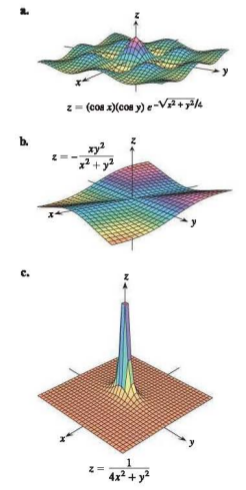
\includegraphics[width=.5\linewidth]{surfaces1.png}
		\end{minipage}%
		\begin{minipage}{.6\textwidth}
		  \centering
		  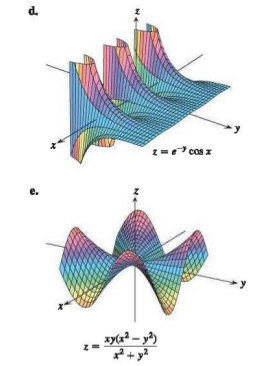
\includegraphics[width=.5\linewidth]{surfaces2.png}
		\end{minipage}
		\end{figure}
		The easiest match is probably that of level curves \textbf{34.} with surface \textbf{c.}. The function is symmetric with respect
		to reflections, does not have local minima and so behave the level curves.\\
		Level curves \textbf{34.} should be matched with the surface \textbf{b.}, as the function is relatively flat (hence many level 
		curves on a picture) with level curves consisting of almost linear pieces as the function does not have strong bends.\\
		Surface \textbf{a.} should be matched to level curves at \textbf{33.}, as function have many local maxima located in rectangular
		grid and level curves near the maxima look like circles, that conveys their "hill-like" shape.\\
		Surface \textbf{d.} should be matched with level curves \textbf{35.}, as it is the only surface that is periodic in $x$-direction
		(due to $\cos x$ multiplier) and non-periodic in $y$.\\
		Surface \textbf{f.} should be matched with \textbf{31.} as function has only two local maxima, unique among the surfaces presented.
		\\
		Finally, \textbf{32.} is matched with \textbf{e.} by elimination.
		}
	\item[\# 54.]{{\it Sketch a typical level surface for the function}\[f(x,y,z)=\ln(x^2+y^2+z^2)\]
		As $\ln:\mysetn{x\in\mathbb{R}}{x>0}\mapsto\mathbb{R}$ is one-to-one and onto, for any $c>0$, $\ln(x^2+y^2+z^2)=c\iff x^2+y^2+z^2=e^c$, hence the typical
		level surface is nothing but sphere $x^2+y^2+z^2=e^c$ in $\mathbb{R}^3$, which looks like \mypic{1.0}{54.jpg}
		}
\end{description}
\end{document}
%Sec. 14.1 # 9, 15, 27, 30, 31-36, 54
